\documentclass[10pt,a4paper]{article}

% Import packages
\usepackage[utf8]{inputenc}
\usepackage{amsmath}
\usepackage{amsfonts}
\usepackage{amssymb}
\usepackage{xcolor}
\usepackage{float}
\usepackage{graphicx}
\usepackage[left=2cm,right=2cm,top=2cm,bottom=2cm]{geometry}

% Inhoud van titelpagina
\author{Quinten Bruynseraede  \\ R0674455 \and Louis Van Looy \\ R0861408}
\title{The Ethereum network: a graph analysis}

% Kolomlayout
\usepackage{multicol}
\setlength{\columnsep}{1cm}

% Gebruik \todo{x} voor rode tekst
\newcommand{\todo}[1]{\textcolor{red}{#1}}
\begin{document}

% Voeg title en authors vanboven in
\maketitle

% Abstract 
\begin{abstract}
	Lorem ipsum dolor sit amet, consectetur adipiscing elit. Vestibulum laoreet dapibus purus. Maecenas eleifend, ipsum eget pretium blandit, nibh diam fermentum turpis, quis semper urna orci eget dolor. Aliquam at vehicula odio. Sed facilisis, odio vitae faucibus consequat, nisi metus condimentum leo, et malesuada sapien metus nec odio. Etiam vel orci non dolor interdum ultricies. Nullam in justo dui. Aenean ut eros non felis molestie lacinia eget ut turpis. Mauris malesuada efficitur libero, at volutpat arcu imperdiet ac. Vivamus gravida sodales felis, varius ultrices magna luctus sit amet. Donec blandit ante neque, at blandit dui vestibulum in. Nam vel lorem. 
\end{abstract}

\begin{multicols}{2}

Een paar handige commando's:
\begin{itemize}
\item{\begin{verbatim}\todo{x}\end{verbatim} Maakt rode tekst: \todo{x}}
\item{\begin{verbatim}\section{sectienaam}\end{verbatim}Maak een nieuwe sectie}
\item{\begin{verbatim}\subsection{sectienaam}\end{verbatim}Maak een nieuwe subsectie}
\item{\begin{verbatim}\textbf{tekst}\end{verbatim}Zet tekst in \textbf{bold}}
\item{\begin{verbatim}\textit{tekst}\end{verbatim}Zet tekst in \textit{italics}}
\item{\begin{verbatim}\cite{referentie-naam}\end{verbatim}Maakt verwijzing naar bron (gedefinieerd in references.bib}
\item{\begin{verbatim}\begin{itemize}
\item{item1}
\item{item2}
\end{itemize}\end{verbatim}Maakt een opsomming met bolletjes}
\item{\begin{verbatim}\begin{enumerate}
\item{item1}
\item{item2}
\end{enumerate}\end{verbatim}Maakt een opsomming met nummers}

\end{itemize}

% Nieuwe sectie met \section
\section{Introduction}
Lorem ipsum dolor sit amet, consectetur adipiscing elit. Vestibulum laoreet dapibus purus. Maecenas eleifend, ipsum eget pretium blandit, nibh diam fermentum turpis, quis semper urna orci eget dolor. Aliquam at vehicula odio. Sed facilisis, odio vitae faucibus consequat, nisi metus condimentum leo, et malesuada sapien metus nec odio. Etiam vel orci non dolor interdum ultricies. Nullam in justo dui. Aenean ut eros non felis molestie lacinia eget ut turpis. Mauris malesuada efficitur libero, at volutpat arcu imperdiet ac. Vivamus gravida sodales felis, varius ultrices magna luctus sit amet. Donec blandit ante neque, at blandit dui vestibulum in. Nam vel lorem.\\

Dit is tekst in \textbf{Bold}, \todo{Rood} of \textit{Italics}.
\section{Ethereum}
% Subsections

In the following section the fundamental terms and definitions to understand the Ethereum network will be granted. Based on this, it is also intended to better understand the network and thus observe and understand the specific characteristics of the particular network. 

\subsection{Ethereum}
First of all a formal definition of Ethereum is needed. Ethereum is an open-source, blockchain-based and decentralized software platform. It makes use of its own cryptocurrency, called ether. It mainly makes it possible to execute Smartcontracts and to create decentralized and distributed applications without any downtime, fraud, control or involvement from a third party. A Smartcontract can be seen as a computer program or transaction protocol created to execute, control or document legally events and actions as set to the terms in an agreement or contract between two parties. Ethereum in not merely a platform, this is as well a programming language that is Turing complete and is operating on blockchain technology (Frankenfield, 2021). 
\subsection{Whales}
A whale
An important element within the composition of the Ethereum network are whales. Ma (2021) gives the following definition: “The term “whale” is used to describe an individual or organization that holds a large amount of a particular cryptocurrency.” This amount is not clearly defined, but within the cryptocurrency community a threshold of around 1.000 of a particular cryptocurrency is being set as the standard. The choice of the name whale is due to the fact that these parts of the network have a lot of market power on the network and are able to push the market up or down. A whale is not especially limited to an individual, this could also refer an institution or organization that holds a significant amount of cryptocurrencies (Ma, 2021).
\subsection{The network}
Lorem ipsum dolor sit amet, consectetur adipiscing elit. Vestibulum laoreet dapibus purus. Maecenas eleifend, ipsum eget pretium blandit, nibh diam fermentum turpis, quis semper urna orci eget dolor. Aliquam at vehicula odio. Sed facilisis, odio vitae faucibus consequat, nisi metus condimentum leo, et malesuada sapien metus nec odio. 
\subsection{Smart contracts}
Etiam vel orci non dolor interdum ultricies. Nullam in justo dui. Aenean ut eros non felis molestie lacinia eget ut turpis. Mauris malesuada efficitur libero, at volutpat arcu imperdiet ac. Vivamus gravida sodales felis, varius ultrices magna luctus sit amet. Donec blandit ante neque, at blandit dui vestibulum in. Nam vel lorem.
\section{Related Work}
	Lorem ipsum dolor sit amet, consectetur adipiscing elit. Vestibulum laoreet dapibus purus. Maecenas eleifend, ipsum eget pretium blandit, nibh diam fermentum turpis, quis semper urna orci eget dolor. Aliquam at vehicula odio. Sed facilisis, odio vitae faucibus consequat, nisi metus condimentum leo, et malesuada sapien metus nec odio. Etiam vel orci non dolor interdum ultricies. Nullam in justo dui. Aenean ut eros non felis molestie lacinia eget ut turpis. Mauris malesuada efficitur libero, at volutpat arcu imperdiet ac. Vivamus gravida sodales felis, varius ultrices magna luctus sit amet. Donec blandit ante neque, at blandit dui vestibulum in. Nam vel lorem.
\section{Analysis of the Ethereum network}
Lorem ipsum dolor sit amet, consectetur adipiscing elit. Vestibulum laoreet dapibus purus. Maecenas eleifend, ipsum eget pretium blandit, nibh diam fermentum turpis, quis semper urna orci eget dolor. Aliquam at vehicula odio. Sed facilisis, odio vitae faucibus consequat, nisi metus condimentum leo, et malesuada sapien metus nec odio. \\
\todo{Eindig een paragraaf met 2 backslashes\\}
Etiam vel orci non dolor interdum ultricies. Nullam in justo dui. Aenean ut eros non felis molestie lacinia eget ut turpis. Mauris malesuada efficitur libero, at volutpat arcu imperdiet ac. Vivamus gravida sodales felis, varius ultrices magna luctus sit amet. Donec blandit ante neque, at blandit dui vestibulum in. Nam vel lorem.
	
\begin{figure}[H]
\centering
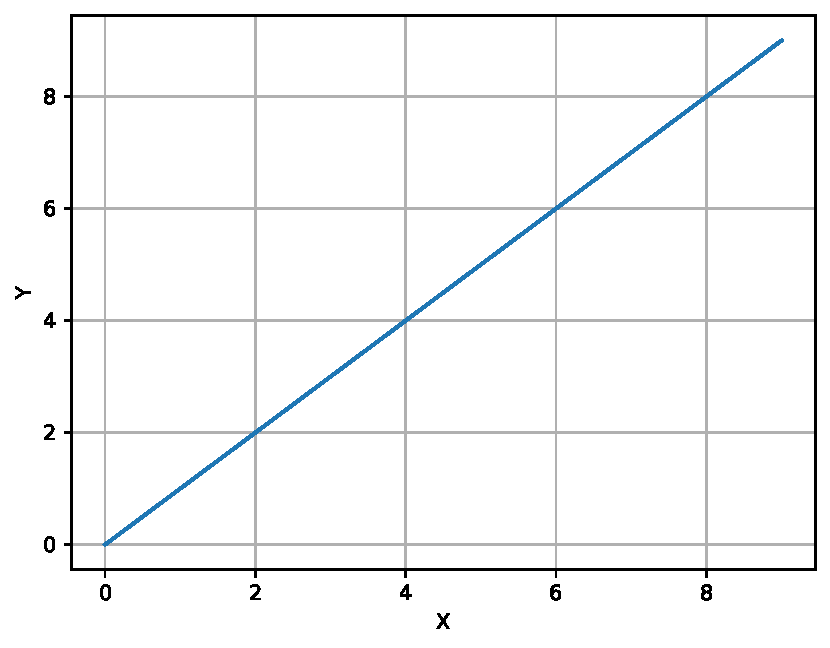
\includegraphics[scale=0.44]{figures/graph.pdf}
\caption{A graph}
\label{fig-agraph}
\end{figure}

Hier verwijs ik automatisch naar Figure \ref{fig-agraph}. \\
\todo{Hier maak ik een citaat, dat komt automatisch in de bibliography vanonder \cite{Becchetti06acomparison}.}
\section{Whales}
	Lorem ipsum dolor sit amet, consectetur adipiscing elit. Vestibulum laoreet dapibus purus. Maecenas eleifend, ipsum eget pretium blandit, nibh diam fermentum turpis, quis semper urna orci eget dolor. Aliquam at vehicula odio. Sed facilisis, odio vitae faucibus consequat, nisi metus condimentum leo, et malesuada sapien metus nec odio. Etiam vel orci non dolor interdum ultricies. Nullam in justo dui. Aenean ut eros non felis molestie lacinia eget ut turpis. Mauris malesuada efficitur libero, at volutpat arcu imperdiet ac. Vivamus gravida sodales felis, varius ultrices magna luctus sit amet. Donec blandit ante neque, at blandit dui vestibulum in. Nam vel lorem.


\end{multicols}
\bibliographystyle{plain}
\bibliography{references}
\end{document}
